\chapter{文本属性设置\label{ch11}}
\section{设置字体属性和文本属性}
字体属性支持 matplotlib.text.Text 实例的属性,也支持函数 matplotlib.pyplot.text()和实例方法 matplotlib.axes.\_axes.Axes.text() 的关键字参数。

\begin{table}
    \centering
    \caption{支持字体属性的函数和实例方法}
    \begin{tabular}{ll}
        \hline
        matplotlib.pyplot API & Matplotlib Object Oriented API            \\
        \hline
        text()                & matplotlib.axes.\_axes.Axes.text()        \\
        xlabel()              & matplotlib.axes.\_axes.Axes.set\_xlabel() \\
        ylabel()              & matplotlib.axes.\_axes.Axes.set\_ylabel() \\
        title()               & matplotlib.axes.\_axes.Axes.set\_title()  \\
        suptitle()            & matplotlib.figure.Figure.suptitle()       \\
        \hline
    \end{tabular}
\end{table}

值得注意的是,字体属性 weight 中的属性值 a numeric value in range 0-1000 和字体属性 size 中的属性值 size in points 都表示实际数值,因此,在代码中作为参数值使用时不需要添加双引号,而其他的字体属性值也包括其他字体属性对 应的字体属性值,在代码中以参数值形式使用时都需要添加双引号,如 family="serif"。

\begin{table}
    \centering
    \caption{配置要素 font 的字体属性和对应的字体属性值}
    \begin{tabular}{l|l|l|l|l|l}
        \hline
        属性 & \textbf{family} & \textbf{style} & \textbf{weight}                 & \textbf{size}  & \textbf{variant} \\
        \hline
        ~  & serif           & normal         & a numeric value in range 0-1000 & size in points & normal           \\
        ~  & sans-serif      & italic         & ultralight                      & xx-small       & small-caps       \\
        ~  & cursive         & oblique        & light                           & x-small        & ~                \\
        ~  & fantasy         & ~              & normal                          & small          & ~                \\
        ~  & monospace       & ~              & regular                         & medium         & ~                \\
        ~  & ~               & ~              & book                            & large          & ~                \\
        ~  & ~               & ~              & medium                          & x-large        & ~                \\
        ~  & ~               & ~              & roman                           & xx-large       & ~                \\
        ~  & ~               & ~              & semibold                        & ~              & ~                \\
        ~  & ~               & ~              & demibold                        & ~              & ~                \\
        ~  & ~               & ~              & demi                            & ~              & ~                \\
        ~  & ~               & ~              & bold                            &                & ~                \\
        ~  & ~               & ~              & heavy                           &                & ~                \\
        ~  & ~               & ~              & extra bold                      &                & ~                \\
        ~  & ~               & ~              & black                           &                & ~                \\
        \hline
    \end{tabular}
\end{table}
\section{延伸阅读:手动添加字体}
\begin{tcolorbox}
    有些字体是付费的,使用请一定注意
\end{tcolorbox}

手动添加字体,具体步骤如下所示:
\begin{enumerate}
    \item 下载需要的字体,例如 New Century Schoolbook Bold.ttf。
    \item 将字体放在字体库 INSTALL/matplotlib/mpl-data/fonts/ttf 中,其中 INSTALL 是类似于 Linux
          平台上的/usr/lib/python3.5/site-packages 和 Windows 平台上的 C:/Python35/Lib/site-packages。
    \item 调用 matplotlib 中的模块 font\_manager,使用模块 font\_manager 中的类 FontProperties(fname),将参数 fname 设定为字体 New Century Schoolbook Bold.ttf 所在的路径 fname="INSTALL/matplotlib/mpl-data/fonts/ttf/New Century Schoolbook Bold.ttf"。
    \item 具体语句是 newfont = matplotlib.font\_manager.FontProperties("INSTALL/matplotlib/mpl-data/fonts/ttf/New Century Schoolbook Bold.ttf "),字体文件名称以属性内容中的名称为主。
    \item 将实例 newfont 作为参数 fontproperties 分别放在显示文本内容的函数中,具体语句 matplotlib.pyplot.xlabel("textContent",fontproperties=newfont) , matplotlib.pyplot.ylabel ("textContent", fontproperties=newfont)。
\end{enumerate}
\begin{figure}
    \centering
    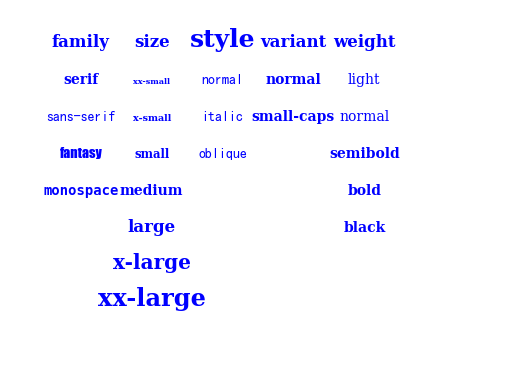
\includegraphics{9787121348884/img/fig11-5.png}
\end{figure}